\chapter{Trabalhos Relacionados}
\label{cap:trabalhos-relacionados}

Integer non lacinia magna. Aenean tempor lorem tellus, non sodales nisl commodo ut. Proin mattis placerat risus sit amet laoreet. Praesent sapien arcu, maximus ac fringilla efficitur, vulputate faucibus sem. Donec aliquet velit eros, sit amet elementum dolor pharetra eget. Integer eget mattis libero

\section{Trabalho Relacionado A}
\label{sec:trabalho-relacionado-a}

Ut accumsan pellentesque feugiat. Sed dui lorem, auctor nec malesuada a, tincidunt at dolor. Donec dapibus velit vitae consequat fringilla. Maecenas egestas, ipsum pellentesque aliquet fringilla, ligula felis luctus erat, eu dapibus dui eros non lacus. Vestibulum accumsan dapibus accumsan. Quisque aliquam nunc id scelerisque tempor. Nullam rhoncus, libero sed varius ullamcorper, velit turpis aliquet metus, et auctor erat purus non felis. Proin quis tempor nisl.

	\begin{figure}[ht!]
		\centering
		\Caption{\label{fig:exemplo-5} Lorem ipsum dolor sit amet, consectetur adipiscing elit. Suspendisse commodo lectus et augue elementum varius.}	
		\UECEfig{}{
			\fbox{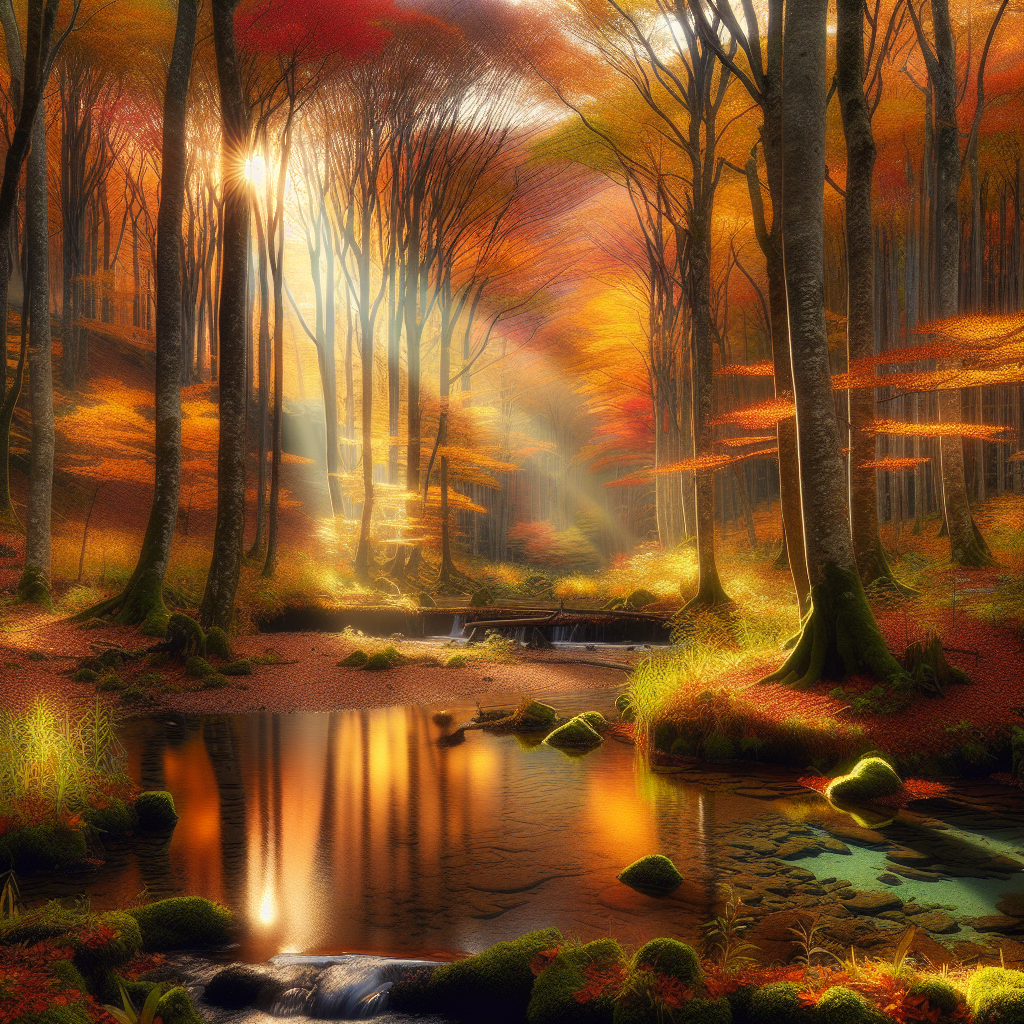
\includegraphics[width=8cm]{figuras/figura-5}}
		}{
			\Fonte{Elaborado pelo autor}
		}	
	\end{figure}
	
Vestibulum accumsan sapien in finibus gravida. Ut semper laoreet turpis. Donec dignissim massa auctor sapien feugiat, a luctus massa viverra. Quisque gravida placerat arcu pharetra auctor. Ut mollis eros nisl, ut viverra nulla convallis vel. Praesent posuere porta lorem eu dictum. Nam faucibus fermentum ex, vitae venenatis tortor condimentum vitae. Mauris massa tellus, molestie at dolor sit amet, ultricies molestie dui. Cras accumsan malesuada quam, ut aliquet mi vulputate sed. Curabitur varius erat id neque porttitor finibus. Donec sed vulputate nunc, ac ultrices augue. Fusce ut commodo eros. Duis lorem erat, finibus in interdum eget, cursus vel quam.

\section{Trabalho Relacionado B}
\label{sec:trabalho-relacionado-b}

Integer non lacinia magna. Aenean tempor lorem tellus, non sodales nisl commodo ut. Proin mattis placerat risus sit amet laoreet. Praesent sapien arcu, maximus ac fringilla efficitur, vulputate faucibus sem. Donec aliquet velit eros, sit amet elementum dolor pharetra eget. Integer eget mattis libero. Praesent ex velit, pulvinar at massa vel, fermentum dictum mauris. Ut feugiat accumsan augue, et ultrices ipsum euismod vitae

	\begin{figure}[ht!]
		\centering
		\Caption{\label{fig:exemplo-4} Maecenas luctus augue odio, sed tincidunt nunc posuere nec}	
		\UECEfig{}{
			\fbox{
\includegraphics[width=8cm]{figuras/figura-4}}
		}{
			\Fonte{Elaborado pelo autor}			
		}	
	\end{figure}

Nunc ac pretium dui. Mauris aliquam dapibus nulla ac mattis. Aenean non tortor volutpat, varius lectus vitae, accumsan nibh. Cras pretium vestibulum enim, id ullamcorper tortor ultrices non. Integer sodales viverra faucibus. Curabitur at dui lacinia, rhoncus lacus at, blandit metus. Integer scelerisque non enim quis ornare.

	\begin{quadro}[ht!]	
		\centering
		\Caption{\label{qua:exemplo-1} Praesent ex velit, pulvinar at massa vel, fermentum dictum mauris. Ut feugiat accumsan augue}		
		\UECEqua{}{
			\begin{tabular}{|c|c|l|l|}
				\hline
				Quisque & pharetra & tempus & vulputate \\
				\hline
				E1 & Complete coverage by a single transcript & Both  & Complete\\
				\hline
				E2 & Complete coverage by more than & Both splice sites & Complete\\
				\hline
				E3 & Partial coverage & Both splice sites & Both \\				
				\hline
			\end{tabular}
		}{
			\Fonte{Elaborado pelo autor}
		}
	\end{quadro}
	
Donec luctus nunc eget mi pellentesque, ac finibus orci placerat. Aenean vestibulum odio at neque tempor convallis. Maecenas elit magna, fringilla consequat lorem id, faucibus dictum turpis. Fusce vel suscipit nunc. Morbi facilisis odio in turpis gravida, eu porta metus ultricies. Sed tincidunt eget nulla eget tempor. Fusce orci velit, posuere in scelerisque a, vehicula sed leo. Phasellus sagittis, mauris id iaculis vehicula, enim diam faucibus nisi, vel condimentum lectus urna id eros. Morbi et ante ligula. Nullam eu dolor eget diam consectetur faucibus eget et lorem. Nam tempor, arcu ut fringilla scelerisque, diam risus molestie metus, ac condimentum nisl diam eu tortor. Aliquam fringilla commodo libero, et mollis mi varius id. Etiam vel vehicula sapien. Cras volutpat eros vehicula, vehicula ex non, sagittis purus. Phasellus pellentesque lacus semper, egestas ante eu, molestie massa. Fusce dictum non justo id viverra.

	
	\begin{quadro}[ht!]	
		\centering
		\Caption{\label{qua:exemplo-2} Duis faucibus, enim quis tincidunt pellentesque}		
		\UECEqua{}{
			\begin{tabular}{|c|c|}
				\hline
				Quisque & pharetra \\
				\hline
				E1 & Complete coverage by a single transcript \\
				\hline
				E2 & Complete coverage by more than \\
				\hline
				E3 & Partial coverage \\
				\hline
				E4 & Partial coverage \\
				\hline
				E5 & Partial coverage \\
				\hline
				E6 & Partial coverage \\
				\hline
				E7 & Partial coverage \\
				\hline
			\end{tabular}
		}{
			\Fonte{Elaborado pelo autor}
		}
	\end{quadro}

Mauris laoreet, turpis et congue mollis, nibh felis mollis ante, a malesuada sapien mauris nec sem. Phasellus nec orci euismod purus auctor viverra auctor vitae nibh. Donec laoreet ante leo, a accumsan dolor convallis et. Donec rutrum nisl ut odio dignissim molestie. Pellentesque vitae diam gravida, convallis nisi sed, dapibus eros. Aliquam consectetur sed nibh vitae rhoncus. In sed ipsum lacus. Suspendisse nulla mi, convallis in arcu eget, consectetur euismod arcu. Maecenas eu tincidunt nisl, non finibus dui. Aliquam lorem lacus, pellentesque in metus eu, placerat ullamcorper metus. Sed condimentum cursus accumsan. Nullam a elementum ex.

Integer non lacinia magna. Aenean tempor lorem tellus, non sodales nisl commodo ut. Proin mattis placerat risus sit amet laoreet. Praesent sapien arcu, maximus ac fringilla efficitur, vulputate faucibus sem. Donec aliquet velit eros, sit amet elementum dolor pharetra eget. Integer eget mattis libero.
\Gls{ambiguidade}
\Gls{braile}
\Gls{coerencia}
\Gls{dialetos}
\Gls{elipse}
\Gls{locucao-adjetiva}
\Gls{modificadores}
\Gls{paronimos}
\Gls{sintese}
\Gls{borboleta}